\section{Real three-symbol alphabets}\label{sec:threesymbol}

The same method works with one more real letter.  Signs are in the alphabet and dividing every
word by a letter does not change the pool, so a real alphabet $\{0,\pm a,\pm b,\pm c\}$ whose
letters have three distinct nonzero absolute values may be written $\{0,\pm1,\pm x,\pm y\}$ with
$1<x<y$; if two absolute values agree or a letter is zero, the alphabet has at most two symbols and
Theorem~\ref{thm:twosymbol} applies.

\begin{theorem}[Real three-symbol alphabets]\label{thm:threesymbol}
Let $1<x<y$ be real and $S(x,y)$ the pool of all words over $\{0,\pm1,\pm x,\pm y\}$.
\begin{enumerate}[label=(\roman*)]
\item $S(x,y)$ is uncolorable if and only if two of the letters $1,x,y$ have ratio $2$ or
$\sqrt2$, or $(x,y)$ is one of the eight points of Table~\ref{tab:threesymbol}.
\item Its minimum uncolorable subset has 31 rays when two letters have ratio~2, 33 rays when two
letters have ratio $\sqrt2$ and none has ratio~2, and between 42 and 57 rays at the eight points
(Table~\ref{tab:threesymbol}).
\item Consequently, if all rays of a KS set have coordinates in $\{0,\pm a,\pm b,\pm c\}$ for some
real numbers $a,b,c$, the set has at least 31 rays.
\end{enumerate}
\end{theorem}

\begin{proof}
An inner product of two words, and a $2\times2$ minor of two words, is
$p_c=c_0+c_1x+c_2y+c_3x^2+c_4xy+c_5y^2$ for an integer vector~$c$ with
$\sum_k|c_k|\le3$; 376 nonzero vectors occur, counting $c$ and $-c$ separately.  Factor each $p_c$ over~$\Q$;
125 distinct irreducible factors appear.  Since $p_c(P)=0$ exactly when one of its factors vanishes
at~$P$, which words are proportional, and hence which words represent the same ray, and which
are orthogonal depend only on the set $F(P)$ of irreducible factors that vanish at~$P$; so
does the orthogonality graph.  The sets $F(P)$ that occur for $P$ in the domain $D=\{1<x<y\}$ are:
the empty set; $\{f\}$ for each factor $f$ whose zero set meets $D$ in a curve (31 of them); and
the set $F(P)$ at each point of $D$ that lies on two of these curves or is a singular point of
one.  There are 130 such special sets.  The script \texttt{ks\_three\_symbol\_real.py} makes
every one of these decisions exactly, holding real algebraic numbers as rational isolating
intervals and deciding signs by exact interval arithmetic.  It finds the curves by cutting the
line $x>1$ at the real roots of the leading coefficient and discriminant in~$y$ and of
$f(x,x)$: on each cell the real branches over~$x$ neither meet nor cross $y=x$, so one rational
point per cell decides whether a branch lies in~$D$.  It finds the special points by splitting
each finite intersection, and the singular locus of each curve, into prime components
$\{(h_x(t),h_y(t)) : q(t)=0\}$ with $q$ irreducible, using a separating coordinate
$t=x+sy$ after making the ideal radical.  A factor $h$ vanishes on a component exactly
when $q$ divides $h(h_x,h_y)$.  It then builds the $1+31+130=162$ graphs and decides
colorability.  As a cross-check it evaluates every special point to 60 digits.  It also
rebuilds the graph (the partition of the words into rays and the set of orthogonal pairs) at a
point of each of the 162 strata, this time from the coordinates and without the factorisation,
and finds it identical in every case.  An earlier version of the scan that made the same
decisions in floating point gave the same 162 cases.

Six curves are uncolorable: $x=2$, $y=2$, $y=2x$, $x^2=2$, $y^2=2$, $y^2=2x^2$.  The generic
point, the other 25 curves and 65 of the special sets are colorable; the other 65 special sets
are uncolorable, and all but eight of them lie on one of the six curves.  Every uncolorable case
was certified (Section~\ref{sec:methods}), each run also proved separately that no
uncolorable subset has fewer than 31 rays, and a minimum set for each case is archived and
checked uncolorable.  Points of the six curves have the minimum of the
curve, except that a point on a ratio-2 curve and a ratio-$\sqrt2$ curve has minimum~31.  This
gives (i) and~(ii).  For (iii), if two of $|a|,|b|,|c|$ agree or one is zero, the set lies in a
two-symbol pool and Theorem~\ref{thm:twosymbol}(iii) applies; otherwise, dividing by the smallest
absolute value and renaming puts it inside some $S(x,y)$.
\end{proof}

\begin{figure}[t]
\centering
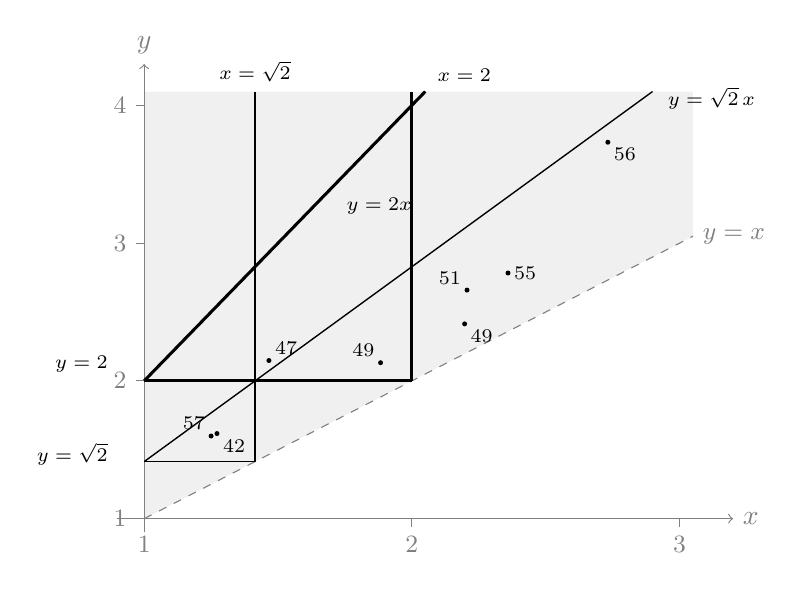
\begin{tikzpicture}[x=3.4cm,y=1.75cm]
\fill[gray!12] (1,1) -- (3.05,3.05) -- (3.05,4.1) -- (1,4.1) -- cycle;
\draw[->,gray] (0.9,1) -- (3.2,1) node[right] {$x$};
\draw[->,gray] (1,0.9) -- (1,4.3) node[above] {$y$};
\foreach \v in {1,2,3} \draw[gray] (\v,1) -- (\v,0.94) node[below,font=\small] {$\v$};
\foreach \v in {1,2,3,4} \draw[gray] (1,\v) -- (0.97,\v) node[left,font=\small] {$\v$};
\draw[gray,dashed] (1,1) -- (3.05,3.05) node[right,font=\small] {$y=x$};
% ratio 2 (minimum 31)
\draw[line width=1.1pt] (2,2) -- (2,4.1);
\draw[line width=1.1pt] (1,2) -- (2,2);
\draw[line width=1.1pt] (1,2) -- (2.05,4.1);
% ratio sqrt 2 (minimum 33)
\draw[line width=0.5pt] (1.4142,1.4142) -- (1.4142,4.1);
\draw[line width=0.5pt] (1,1.4142) -- (1.4142,1.4142);
\draw[line width=0.5pt] (1,1.4142) -- (2.899,4.1);
\node[font=\scriptsize,anchor=south west] at (2.06,4.1) {$x=2$};
\node[font=\scriptsize,anchor=south] at (1.4142,4.1) {$x=\sqrt2$};
\node[font=\scriptsize,anchor=north west] at (1.72,3.4) {$y=2x$};
\node[font=\scriptsize,anchor=west] at (2.92,4.05) {$y=\sqrt2\,x$};
\node[font=\scriptsize,anchor=east] at (0.9,2.12) {$y=2$};
\node[font=\scriptsize,anchor=east] at (0.9,1.47) {$y=\sqrt2$};
% the eight further points, labelled by their minimum
\foreach \px/\py/\m/\a in {1.272/1.618/42/north west, 1.466/2.148/47/south west,
  1.883/2.132/49/south east, 2.197/2.414/49/north west, 2.206/2.659/51/south east,
  2.359/2.783/55/west, 2.732/3.732/56/north west, 1.250/1.600/57/south east}
  {\fill (\px,\py) circle (0.9pt); \node[font=\scriptsize,anchor=\a,inner sep=2pt] at (\px,\py) {\m};}
\end{tikzpicture}
\caption{Real three-symbol alphabets $\{0,\pm1,\pm x,\pm y\}$, $1<x<y$ (shaded).  The pool is
uncolorable exactly on the six lines and at the eight points (Theorem~\ref{thm:threesymbol}).
Heavy lines: two letters have ratio 2, minimum 31.  Light lines: ratio $\sqrt2$, minimum 33
(31 where a light line meets a heavy one).  Each point is labelled with its minimum
(Table~\ref{tab:threesymbol}); the points labelled 42 and 57 are distinct but close.}
\label{fig:threesymbol}
\end{figure}

\begin{table}[t]
\centering
\caption{The eight points of Theorem~\ref{thm:threesymbol} that lie on none of the six
uncolorable curves, with the relations that hold there (each point is the unique point of $D$
satisfying them) and the certified minimum.  Rays, pairs and triads are those of the raw pool.}
\label{tab:threesymbol}
\small
\begin{tabular}{@{}llrrrr@{}}
\toprule
Relations & $(x,y)\approx$ & Rays & Pairs & Triads & Min \\
\midrule
$x^2=y,\ y^2=y+1$\ \ ($x=\sqrt\varphi,\ y=\varphi$) & $(1.272,1.618)$ & 109 & 312 & 28 & 42 \\
$x^3=x^2+1,\ y=x^2$\ \ ($x=\psi,\ y=\psi^2$) & $(1.466,2.148)$ & 109 & 348 & 40 & 47 \\
$y^2=x^2+1,\ xy=x+y$ & $(1.883,2.132)$ & 145 & 474 & 42 & 49 \\
$y^2=x^2+1,\ x^2=2y$\ \ ($y=1+\sqrt2$) & $(2.197,2.414)$ & 145 & 402 & 46 & 49 \\
$xy=x^2+1,\ y=x^2-x,\ y^2=x^2+x$ & $(2.206,2.659)$ & 145 & 462 & 46 & 51 \\
$xy=x^2+1,\ x^2=2y$ & $(2.359,2.783)$ & 145 & 414 & 58 & 55 \\
$y=x+1,\ x^2=2y$\ \ ($x=1+\sqrt3$) & $(2.732,3.732)$ & 145 & 486 & 46 & 56 \\
$xy=2,\ y^2=x^2+1$ & $(1.250,1.600)$ & 145 & 390 & 46 & 57 \\
\bottomrule
\end{tabular}
\end{table}

Three remarks.  First, the curves contribute nothing new: on a ratio-2 curve the pool contains
the words over $\{0,\pm1,\pm2\}$ (after rescaling) and hence $\CK$, and on a ratio-$\sqrt2$ curve
it contains Peres's set; the theorem says that no third letter, placed anywhere on these curves,
gives a smaller set.  Second, the eight points are exceptional uncolorable alphabets (we have
not searched the literature for them), and all their minima exceed~33.  One of them is the supergolden alphabet of Section~\ref{sec:catalogue}, whose
minimum 47 was certified there independently.  Third, the theorem is about real letters; the
complex three-symbol case has the same finite structure in principle but a parameter space of four
real dimensions, and we have not attempted it.
